%%%% CAPÍTULO 1 - INTRODUÇÃO
%%
%% Deve apresentar uma visão global da pesquisa, incluindo: breve histórico, importância e justificativa da escolha do tema,
%% delimitações do assunto, formulação de hipóteses e objetivos da pesquisa e estrutura do trabalho.

%% Título e rótulo de capítulo (rótulos não devem conter caracteres especiais, acentuados ou cedilha)
\chapter{Introdução}\label{cap:introducao}

Um sinal biomédico, ou biossinal, é qualquer quantidade variante no tempo que seja mensurável e relacionada diretamente como efeito de um processo biológico. Esses sinais são utilizados amplamente para analisar as condições e estado de funcionamento de sistemas biológicos de um ser vivo \cite{BiosignalsAndCompressionStandards}. Seu uso na medicina como meio de estudo e diagnóstico de enfermidades é altamente difundido. Alguns exemplos de biossinais são o eletrocardiograma (ECG) para analisar a atividade elétrica do miocardio, ou o sistema cardíaco, o eletroencefalograma (EEG) para avaliar atividades elétricas decorrentes do encéfalo, podendo auxiliar no processo de diagnóstico de determinadas doenças neurológicas e a eletromiografia (EMG) para análise da ativação dos tecidos musculares do corpo.

A redução do custo de produção dos componentes eletrônicos usados na construção de sensores utilizados na captura de biossinais tem fomentando a criação de dispositivos baratos e acessíveis, aumentando o potencial da pesquisa acadêmica em um meio que era restrito devido aos altos custos envolvidos no desenvolvimento e produção desses equipamentos \cite{StorageofBiomedicalSignals}. Esses dispositivos geram um grande volume de dados relevantes para a pesquisa com aprendizado de máquina (ML), porém a natureza heterogênea dos dados dificulta a integração dos mesmos entre diferentes projetos, reduzindo a capacidade de aproveitamento dos dados adquiridos por falta de um processo conhecido e difundido para tratá-los na comunidade científica \cite{ExtensibleBiosignalMetadata}.

Existem várias propostas de semântica e estruturação de dados disponíveis \cite{StorageBIT,BioSignalMLMetaModel}, porém existe uma escassez de trabalhos que construam um processo de troca e armazenamento de dados normalizados entre projetos e instituições de pesquisa clínico-hospitalar sem que isso envolva um grande esforço dos laboratórios em estudar as propostas dos projetos e implementar uma versão própria do artefato que muito provavelmente não segue todas as regras de outra versão desenvolvida por outro laboratório. A falta de abundância desses artefatos prontos para implementação em poucos passos, que forneçam uma infra estrutura de processos e protocolos de tratamento de dados médicos e hospitalares, que forneçam bases para construção de projetos internos e sejam amplamente difundidos entre a comunidade científica e técnica é fonte de complexidade na pesquisa e desenvolvimento de novas soluções. Esse cenário resulta na construção de sistemas específicos com bases de dados desconexas, gerando carga de trabalho extra em normalização e processamento dessas informações para o uso em pesquisas. Essa prática se torna uma fonte de custo, complexidade, risco de inconformidade e pode inviabilizar o processo de extração e normalização de dados de múltiplas fontes.

Quando a pesquisa envolve o ambiente clínico hospitalar, grande parte do esforço envolve organização, garantia de conformidade e gestão das informações disponibilizadas pelos envolvidos. Um desafio apresentado na integração de datasets médicos existentes é o fato de eles serem "pequenos e confinados a silos de dados isolados, recheados de erros de rotulação e viés" \cite{ResponsibleandRegulatoryConformMachineLearning}, efeito da falta de processos difundidos para o tratamento de registros e metadados das informações médicas adquiridas. A falta de padrões adequados significa que, por vezes, arquivos CSV (valores separados por vírgula) foram usados para armazenar e trocar dados de sinais, resultando na perda de metadados armazenados por falhas humanas no processo de gestão dessas informações\cite{ExtensibleBiosignalMetadata}. 

Sendo assim, parte significativa do esforço é despendida no processo de obtenção e normalização das anotações de laboratório dos projetos, que normalmente não compartilham nem de estrutura e nem de semântica, aumentando o tempo de pesquisa e podendo até inviabilizá-la devido à perda de informações por falta de diretivas compartilhadas entre instituições e projetos \cite{BioSignalMLMetaModel}. A figura \cite{fig:exemplo1} ilustra o fluxo de dados em projetos de pesquisas de biossinais.

\begin{figure}[htb]%% Ambiente figure
    %\captionsetup{width=0.55\textwidth}%% Largura da legenda
    \caption{Exemplo de fluxo de consumo de dados em pesquisa envolvendo biossinais}%% Legenda
    \label{fig:exemplo1}%% Rótulo
    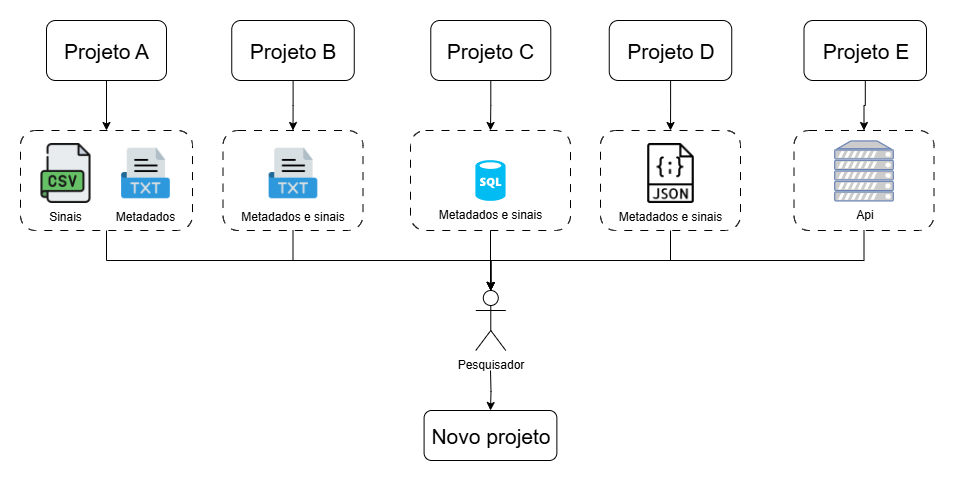
\includegraphics[scale=0.4]{figuras/introducao/exemplo-atual-fluxo-de-trabalho.png}%% Dimensões e localização
    \fonte{Autoria própria (2025)}%% Fonte
\end{figure}

Esse deficit de diretivas é extremamente danoso, pois, além de todas as dificuldades que causa no processo de pesquisa e desenvolvimento, lança desconfiança sobre sistemas e soluções construídas a partir dos dados extraídos. Esse fato dificulta a aceitação e difusão de projetos que se baseiam na sintetização de informações presentes em grandes quantidades de dados, como o caso de soluções desenvolvidas a partir de ML.

O financiamento de pesquisas de desenvolvimento e a difusão de soluções que usam ML na área de engenharia biomédica é dependente da capacidade das mesmas de se provarem confiáveis, seguras e robustas para uso clínico. O método de ML exige acesso a uma grande quantidade de dados representativos e de alta qualidade para atingir os resultados esperados, principalmente devido à alta dimensionalidade do espaço de entrada do domínio que normalmente possuem.

Para que modelos baseados em ML possam realizar inferências confiáveis, é extremamente necessário que esteja disponível para o seu desenvolvimento uma amostra significativa e diversificada para evitar que o sistema sofra com vieses. Na prática, é provado que o desempenho de sistemas baseados em IA está vinculado à qualidade dos dados usados para treinamento \cite{TheEffectsofDataQuality}. Mesmo quando o desempenho esperado é alcançado, a explicabilidade do resultado é prejudicada, afetando a confiança e transparência da utilização do modelo pela comunidade médica, tornando-se o principal desafio a garantia de qualidade dos dados oferecidos para o treinamento do modelo.

Dado a situação atual, uma proposta de diretivas aplicadas para a organização, requisitos e integração de sistemas e projetos de pesquisa biomédicos se mostra fundamental para fomentar o compartilhamento de bases de dados médicas normalizadas entre projetos e instituições, possibilitando a criação de silos de dados médicos semânticos e facilmente integráveis, que por sua vez, reduzem custos e tempo na construção de data bases de dados com múltiplas fontes relacionados ao processo de normalização. Buscando cumprir essa proposta, o presente trabalho apresenta o Padrão de Rótulos e Interfaces para Sistemas Médicos (PRISM), uma série de requisitos e processos esperados de um projeto de pesquisa clínica que orquestra a comunicação entre dois ou mais Nós de Pesquisa Interoperáveis.

\begin{figure}[htb]%% Ambiente figure
    %\captionsetup{width=0.55\textwidth}%% Largura da legenda
    %\caption{Exemplo de fluxo de pesquisa envolvendo biossinais}%% Legenda
    \label{fig:introducao-proposta}%% Rótulo
    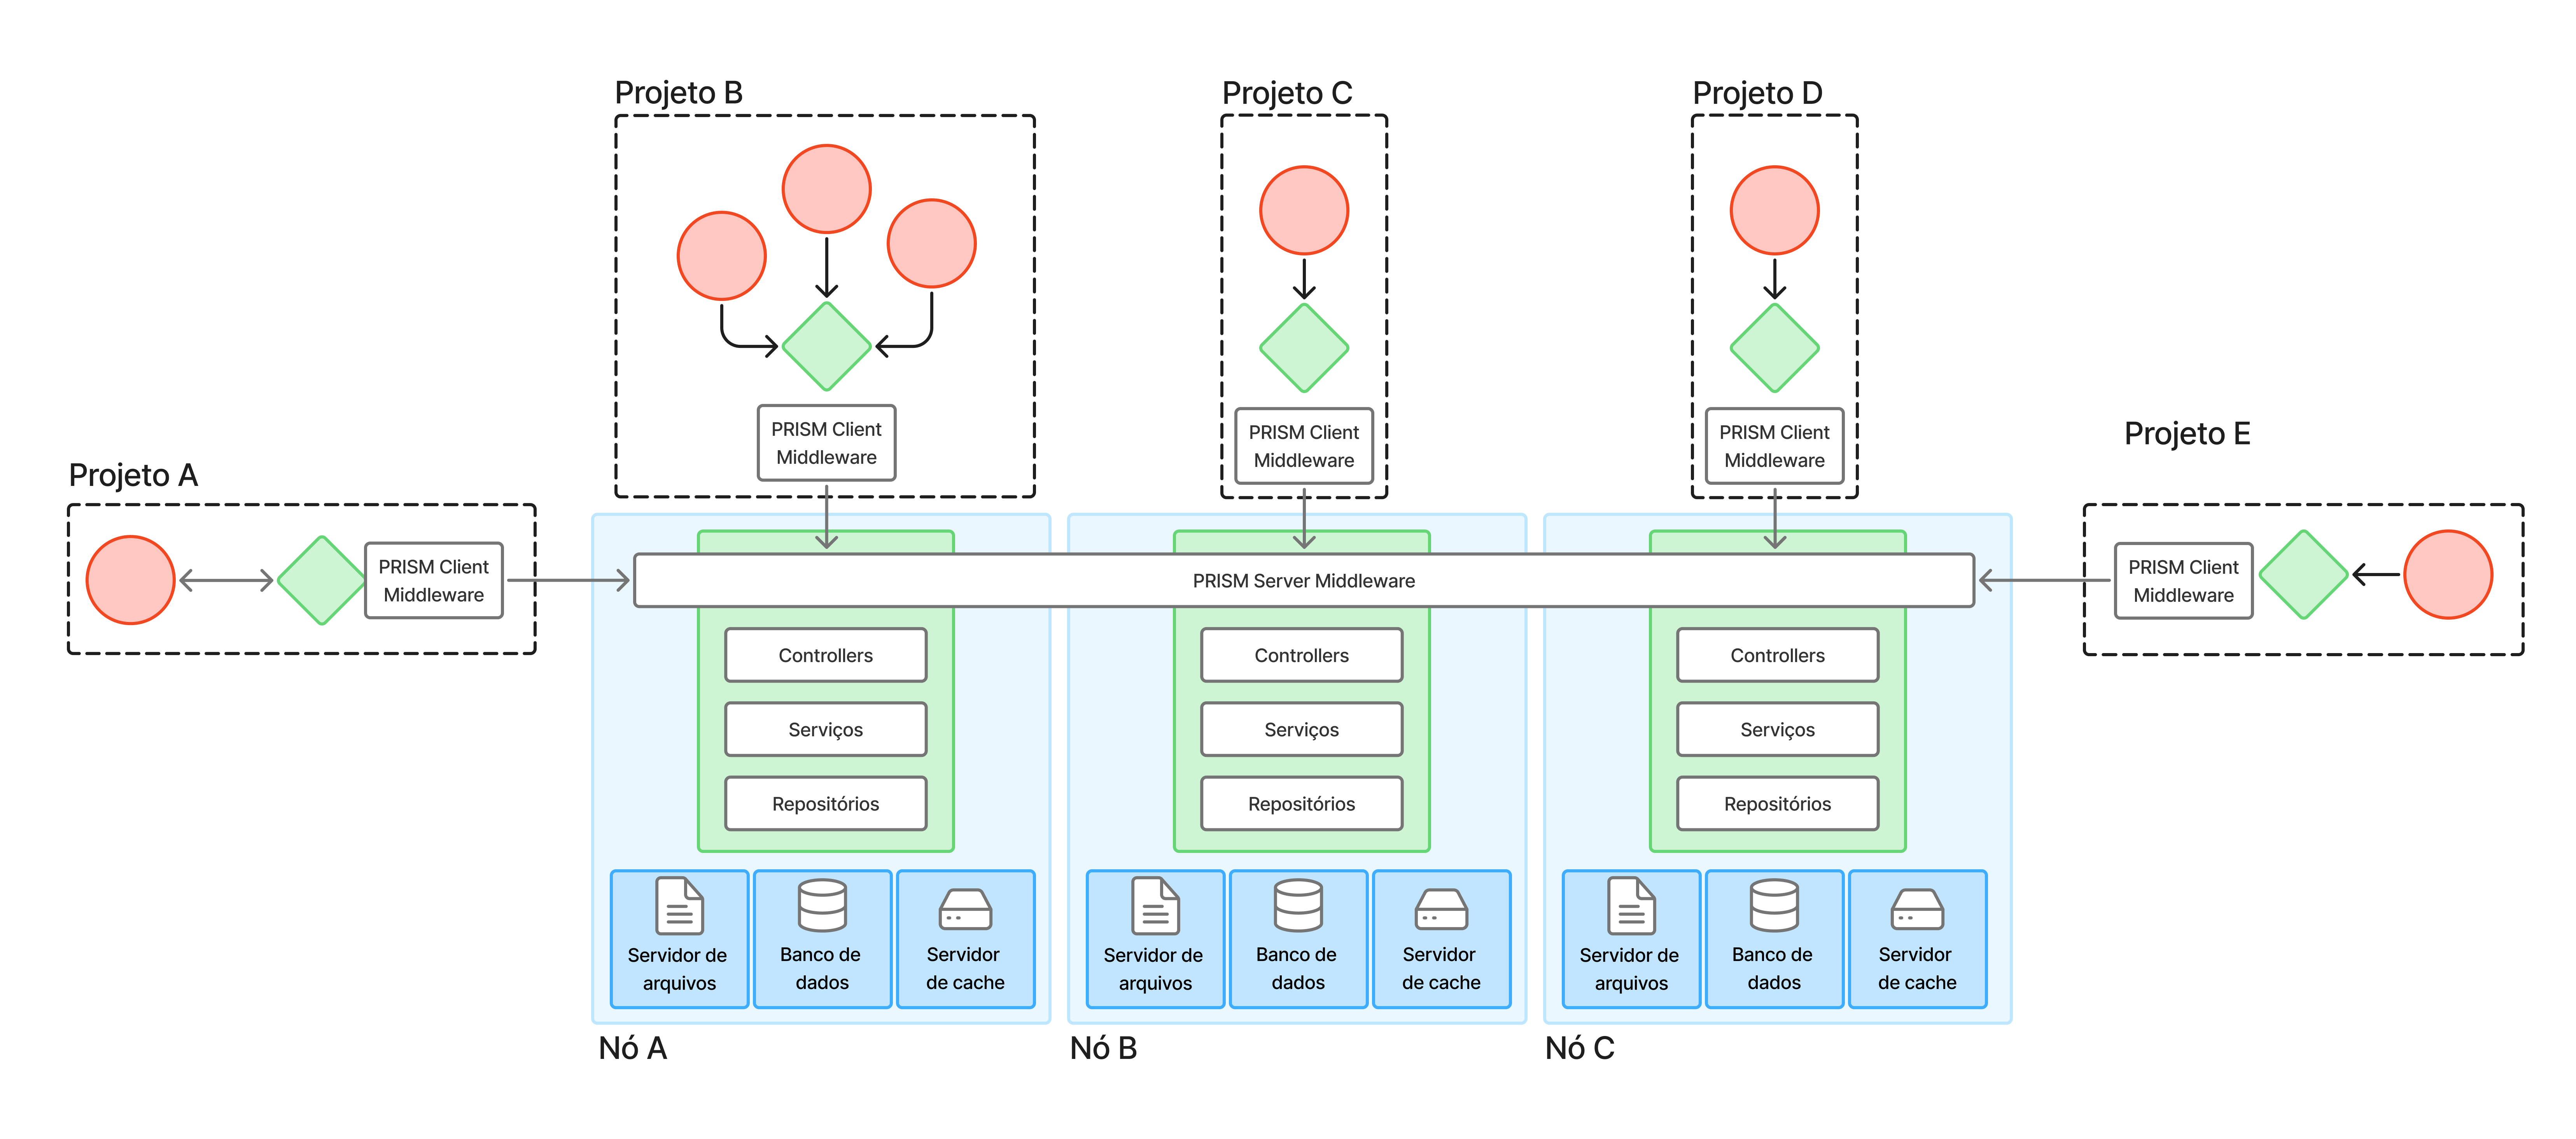
\includegraphics[scale=0.15]{figuras/introducao/proposta.png}%% Dimensões e localização
    \fonte{Autoria própria (2025)}%% Fonte
\end{figure}

\section{Objetivos}\label{sec:objetivos}

O objetivo geral deste trabalho é desenvolver uma padronização de rótulos e interfaces de comunicação de pesquisas clínico-hospitalares, tendo como aplicação de teste um sistema de captura de sinais eletromiografia de superfície existente.

\subsection{Objetivos específicos}\label{subsec:objetivosEspecificos}

\begin{itemize}
  \item Revisar literatura e estado da arte na troca de registros clínicos, biossinais e ontologias entre projetos
  \item Desenvolver um Nó de Pesquisa Aplicada (NPI)
  \item Modificar, adaptar e integrar um projeto de captura de eletromiografia de superfície ao NPI
  \item Testar o resultado final da integração
  \item Avaliar resultados obtidos
\end{itemize}

\section{Metodologia de Pesquisa}\label{sec:MetodologiaDePesquisa}

Essa pesquisa se enquadra como pesquisa aplicada, pois busca desenvolver um artefato que solucionem a dor levantada pelo autor após revisão da literatura sobre o assunto.

\section{Estado da Arte}\label{sec:estadoDaArte}

Existem várias padronizações e plataformas que buscam solucionar a dor levantada pelo autor deste trabalho, principalmente de instituições governamentais, pois é de interesse público o compartilhamento dessas informações para evitar a duplicata de informações do paciente, requisição de exames e melhorar o atendimento disponível ao paciente. O presente trabalho realizou uma pesquisa bibliográfica em sites institucionais, \textit{Google Scholar} e  Periódicos da Coordenação de Aperfeiçoamento de Pessoal de Nível Superior (CAPES) sobre iniciativas governamentais e pesquisas acadêmicas sobre a integração de bancos de dados de informações médicas, com a delimitação do período de 2015 até 2025. Dentre os trabalhos encontrados, destacam-se:
\begin{itemize}
  \item \citeonline{RDNS}, a Rede Nacional de Dados em Saúde(RDNS) é uma plataforma de interoperabilidade público-privada centralizada gerenciada pelo Departamento de Informática do SUS(DATASUS), cujo objetivo descrito pela plataforma é "estabelecer a infraestrutura nacional para o compartilhamento seguro e padronizado de dados de saúde, garantindo mais eficiência na gestão da informação e aprimorando a qualidade dos serviços prestados à população" \cite{RDNS}. Dentre esses dados, se encontram informações demográficas do paciente, histórico de vacinação, prescrição de medicamentos, exames e histórico de vacinas. Seguindo as diretrizes da Lei Geral de Proteção de Dados(LGPD), a RNDS busca disponibilizar de forma segura para profissionais de saúde o histórico clínico do paciente entre as entidades médicas participantes da rede. A integração com a rede por instituições privadas é incentivada através do abatimento de impostos por serviços prestados para o SUS pelo compartilhamento das informações da instituição com a RNDS;
  \item \citeonline{USCDI}, United States Core Data for Interoperability (USCDI) é uma norma que define a estrutura de interoperabilidade entre sistemas médicos que substitui sua antiga versão, a  Common Clinical Data Set(CCDS). Trazendo uma visão de "data-first", ele descreve como os sistemas devem estruturar e transmitir as informações entre si. Diferente do exemplo brasileiro, não existe uma centralização dos dados em um servidor e o modelo se baseia na premissa de certificação dos sistemas interessados. Anualmente o USCDI é revisado, adicionando e removendo informações da estrutura, e no momento de escrita deste trabalho, está em sua 6ª versão;
  \item \citeonline{EHDS}, European Health Data Space Regulation (EHDS) é uma série de regulações políticas e  técnicas sendo implementadas até 2027 que buscam formar uma rede federada para criar um prontuário médico unificado entre países-membros da União Europeia(UE) e fomentar a pesquisa através da distribuição e fiscalização de uso das informações coletadas. Ela define o uso primário dos dados como prover saúde para os pacientes através do fácil acesso de todas as suas informações médicas e continuidade de tratamento pelos países membros da união e o uso secundário como pesquisa e interesse público para políticas pública. "Leis Europeias compartilhadas definem quem pode disponibilizar quais dados disponíveis para quais propósitos e sob quais condições" \cite{EHDS_Implementation_and_governance}. EHDS Board tem todos os países-membros representados, aprimorando o EHDS e regulando a atuação das Autoridades de Saúde Digital nacionais responsáveis pela aplicação do modelo a nível nacional, possibilitando que cada país faça sua implementação das regulações estabelecidas de forma independente, mas obrigue a integração entre as entidades participantes;
  \item \citeonline{NHS} é a abordagem do Reino Unido gerenciada pelo National Health System(NHS). NHS Data Model and Dictionary Service é uma padronização que determina estruturas e requisitos necessários para que qualquer aplicação que interaja com sistema de saúde nacional. Ela assegura a interoperabilidade semântica entre os sistemas participantes através da adoção da terminologia clínica SNOMED CT \cite{SNOMEDCT,SNOMEDCTOverview} para todas as informações clínicas capturadas;
  \item \citeonline{SharedPan-CanadianInteroperability} é o plano canadense para promover a interoperabilidade entre suas províncias. Canada Health Infoway é uma organização federal do governo formada em 2001 com a missão de integrar digitalmente os membros da federação canadense, que sofriam com a fragmentação de seus sistema de saúde. O \textit{Connected Care for Canadians Act}  é um passo com regulações importantes sobre tratamentos de dados médicos pois "requer que qualquer empresa de TI que preste serviços de saúde digital no Canadá adote padrões comuns e permita troca de informação de forma protegida e segura entre vários sistemas"\cite{ConnectedCareAct};
  \item \citeonline{MyHealthRecord} My Health Record é a plataforma de registros médicos digitais australianos. A estratégia do governo é composta por um modelo híbrido em que é oferecido uma plataforma de interoperabilidade e um padrão de dados, o \textit{Australian Core Data for Interoperability}(AUCDI) \cite{AustralianCoreDataforInteroperability} que define quais e como esses dados devem circular pela rede.
\end{itemize}


https://medinform.jmir.org/2022/4/e35789/

https://ebooks.iospress.nl/doi/10.3233/SHTI210070

https://link.springer.com/article/10.1186/s12911-019-0806-z